\section{Intelligence}
Finally, when we have collected all the information, we can start to connect
the pieces more precisely. This is the main component of OSINT and brings out
the actual value. In OSINT, the term "{\bf intelligence}" has a different
definition than the basic definition used by psychologists in the scientific
world. Since there are many disagreements in the definition of "intelligence,"
scientists try to follow a more modern approach, which is described as
follows:

Modern research focuses on information processing. How well, how fast, how long
does someone need to process information, impressions, and stimuli. How quickly
can they retrieve this information? In this context, intelligence is not seen
as a fixed entity but as a variable and, consequently, as a process. How does
the brain process all the information that comes at us? How well do the
cognitive abilities function?

Here, an essential role is played by three different elements:
\begin{verbatim}
Origin =>	Impact => State
\end{verbatim}

Since there is neither a fixed definition for "intelligence" nor a precise
definition explicitly for OSINT, we define it as follows:

{\bf Based on the fact that every state has an origin and an impact, the term
    "intelligence" in OSINT consists of the ability to find out and link the
connections between these elements with the information found.}

In this way, we process information from the past and present to assess the
effects in the future. By analyzing the present information and the changed
conditions with the past, the main focus is on the significant factors for the
present condition. If a company was hacked ({\bf origin}) in the past and there
is no detected intrusion at the moment, it can be determined that the {\bf
impact} has brought about a change in the {\bf state}. The {\bf connections}
between these elements represent a step-by-step process that shows the way in
which the past state has been changed.

\begin{figure}
  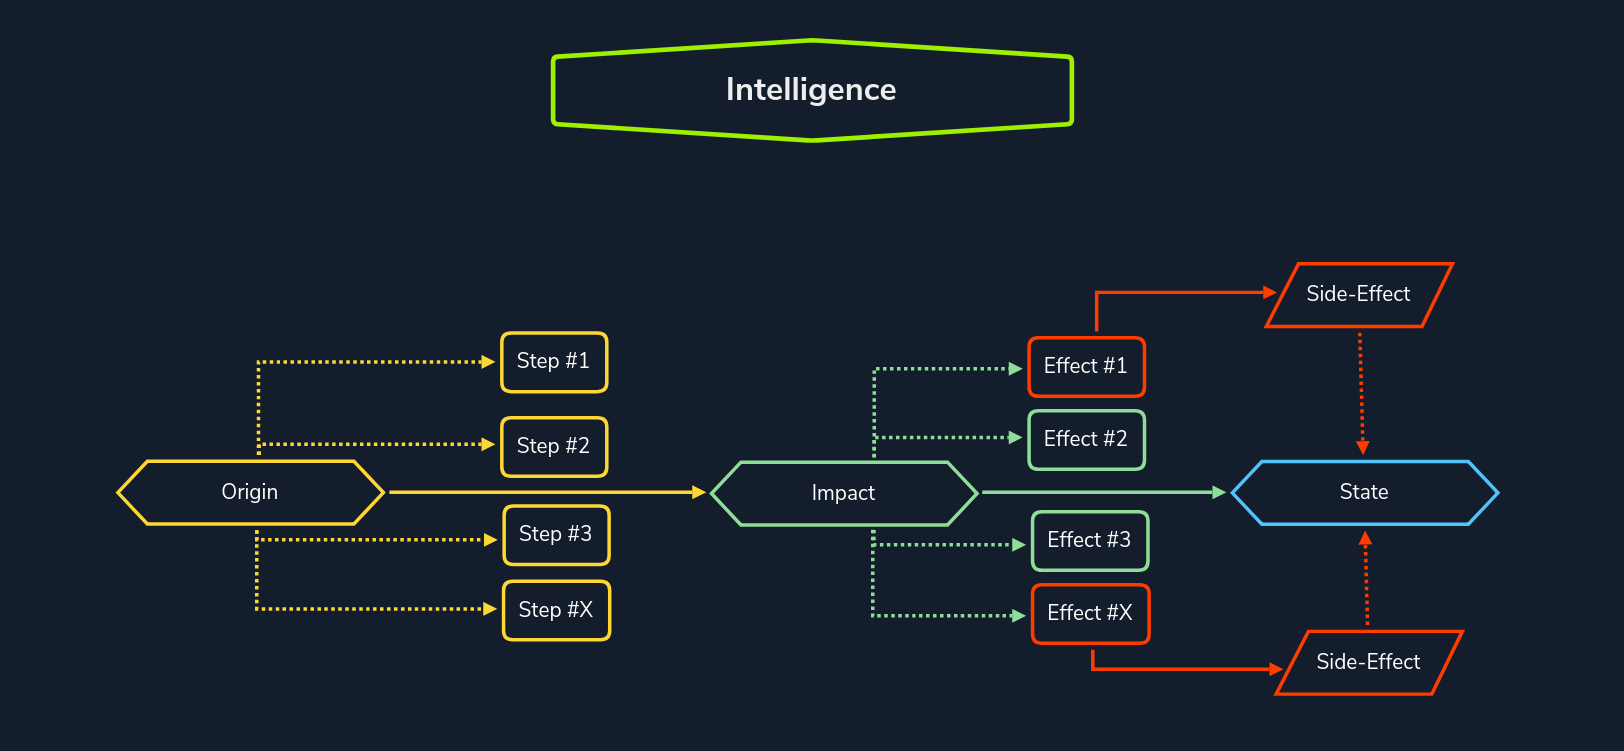
\includegraphics[width=\linewidth]{recon/osint/images/intelligence1.png}
  \caption{OSINT Intelligence}
  \label{fig:osint-intelligence}
\end{figure}

\subsubsection{Origin}
{\bf Each origin refers to an activity carried out in the past with the aim of
changing the future state through some particular impact.}

This means that each activity has a purpose and goal to be achieved. For us,
the necessary steps for this are essential. Therefore, we try to determine
which actions had to be taken to cause the desired impact to reach the current
state. Even if we do not know the state, we can use the steps to calculate its
impact and required actions to achieve the desired state.

\subsubsection{Impact}

To cause or provoke an impact, we need the combination of purpose or goal with
the corresponding action. The goal alone has no direct effect on the desired
state, just as little as an arbitrary action without a goal. Because with the
second, the result would lead to a random state. The steps that need to be
taken depend on the {\bf environment} and {\bf information}. Therefore, to
calculate the impact, we need information about the current state and the
environment in which our target is located. Accordingly, we gain insight into
the dependent factors by which we can calculate step-by-step which actions have
to be executed to achieve the desired state's corresponding impact.

\subsubsection{State}

A state is the result and functioning of different goals and the actions that
have been taken to achieve them. The achievement of a particular state always
automatically leads to {\bf side-effects}. These side-effects are unintended
impacts on the object and/or its environment.

Especially in information security, side-effects define exactly the
component/vulnerability we try to detect during our penetration tests. We can
say that no security-conscious administrator wants to make their company's
network vulnerable or put it at risk. The misconfigurations caused by those
side-effects of the actions to achieve the desired state and functionality are,
in most cases, unintentional. These are precisely the flaws that we as
penetration testers use to uncover these vulnerabilities in combination with
our objectives (simulation of an attacker) and the actions based on an example
(in a penetration test), which impact these can have on the company.

\subsubsection{Next Steps}

During our OSINT investigation, we only have information on the different
conditions for different periods. To understand the impact between two
different states and thus discover the potential side-effects, we need to
recreate the individual steps between impact and state as best as possible by
linking the information gathered.

As an example, we can take a simple software update. In simple terms, an update
is an improvement of the existing software and its version. Thus, the old
version would be the origin, and the new one would be the current state. The
developers had set themselves individual goals before developing a new version,
improving the service, or closing specific security vulnerabilities or bugs.
The individual steps represent the development process in which the code is
renewed, expanded, and improved. Each change (action) to the code has an impact
on the entire software. This can be new functions or improved performance.
However, this can lead to new errors and bugs, representing the side-effects we
want to discover.

Therefore, the art is to track these single steps and, in the best case, as
many as possible. To do this, we need to put ourselves in the administrator's
shoes as best we can. This is also the role of the feedback left by employees,
discovered during our investigation. This feedback gives us an impression of
the working atmosphere and its conditions. A lousy atmosphere leads to
dissatisfaction, demotivation, carelessness, and finally to mistakes that we
try to discover. Once we have found which side-effects have arisen or could
have arisen, we gain an accurate picture of how the software works and thus an
understanding of what actions we need to take to achieve our desired state of
the software.
